\documentclass[11pt, oneside]{article}   	% use "amsart" instead of "article" for AMSLaTeX format
\usepackage{geometry}                		% See geometry.pdf to learn the layout options. There are lots.
\geometry{letterpaper}                   		% ... or a4paper or a5paper or ... 
%\geometry{landscape}                		% Activate for for rotated page geometry
%\usepackage[parfill]{parskip}    		% Activate to begin paragraphs with an empty line rather than an indent
\usepackage{graphicx}				% Use pdf, png, jpg, or eps� with pdflatex; use eps in DVI mode
								% TeX will automatically convert eps --> pdf in pdflatex		
\usepackage{amssymb}
\usepackage{amsmath}
\usepackage{color}

\title{Archimedes}
%\author{The Author}
\date{}							% Activate to display a given date or no date

\graphicspath{{/Users/telliott_admin/Dropbox/Tex/png/}}
\begin{document}

\maketitle
%\section{}
% \subsection*{R code}
% \begin{lstlisting}  \end{lstlisting}
% \begin{center} 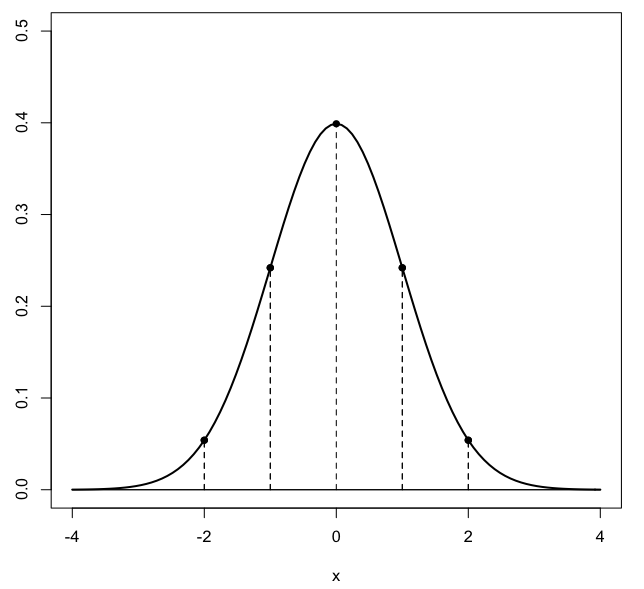
\includegraphics [scale=0.4] {gauss3.png} \end{center}
% \begin{bmatrix} a  &  b \\ c  &  d \end{bmatrix}
% \bigg |_

\large
\noindent In this write-up I want to discuss Archimedes' tremendous discovery about volumes.  He found a connection between the volume of the sphere, the cone and the cylinder, and was so proud of what he discovered that he had the sphere and cylinder engraved or somehow mounted on his tombstone.  Cicero searched for his grave and confirmed the description of the monument nearly 150 years later.

\begin{center} 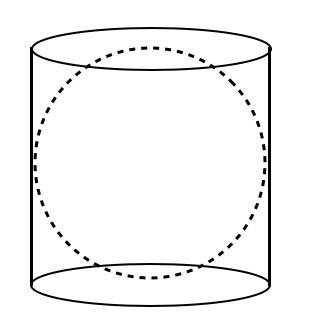
\includegraphics [scale=0.4] {sphere_cyl.png} \end{center}

Perhaps most interesting, Archimedes said that he discovered the correct result by balancing the three objects on a fulcrum.  
\begin{center} 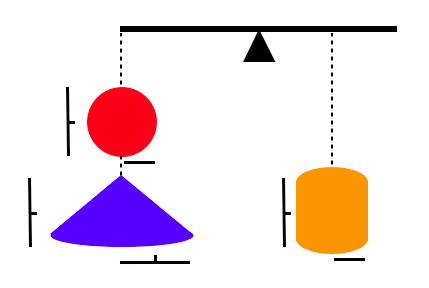
\includegraphics [scale=0.4] {archimedes1.png} \end{center}
We will analyze this figure a bit later.  

According to Archimedes (in the Method, translation by Heath)

\begin{quote}For certain things which first became clear to me by a mechanical method had afterward to be demonstrated by geometry...\textcolor{blue}{it is of course easier, when we have previously acquired by the method some knowledge of questions, to supply the proof than it is to find the proof without any previous knowledge.} This is a reason why, in the case of the theorems the proof of which Eudoxus was the first to discover, namely, that the cone is a third part of the cylinder, and the pyramid a third part of the prism, having the same base and equal height, we should give no small share of the credit to Democritus, who was the first to assert this truth...though he did not prove it.
\end{quote}

Let's consider the first figure shown above.  Start with a sphere of radius $R$, which just fits inside a cylinder, also with radius $R$ and height $2R$.  

\begin{center} 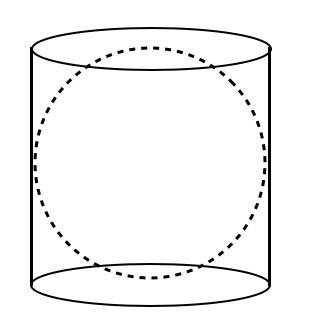
\includegraphics [scale=0.4] {sphere_cyl.png} \end{center}

The volume of this cylinder is 
\[ V_{cylinder} = H \ \pi R^2 = 2R \ \pi R^2 = 2 \pi \ R^3 \]
The volumes of a sphere and cone are
\[ V_{sphere} = \frac{4}{3} \ \pi R^3 \]
\[ V_{cone} = \frac{1}{3} \ \pi R^3 \]
Thus, for this special cylinder and sphere
\[ V_{cylinder} = V_{sphere} + 2 V_{cone} \]
where the cone is one with a radius and height of $R$.

So what I would like you to do is to picture that sphere, with radius $R$, just fitting into a cylinder with radius $R$ and total height $2R$, and beside it a cone, and on top of that an inverted cone.  This pair of cones have a base that is the same as the base of the cylinder (and the central cross-section of the sphere), that is, a circle with radius $R$.

Here is the top half of the picture.

\begin{center} 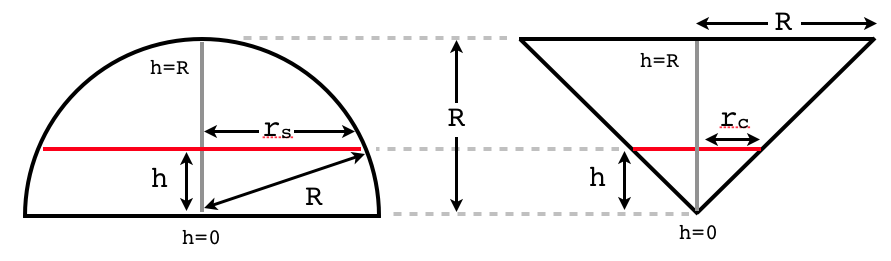
\includegraphics [scale=0.5] {sphere_cone.png} \end{center}

According to our formulas, the volume of the cone is
\[ V_{cone} = \frac{1}{3} \ H \ \pi R^2 = \frac{1}{3} \ R \ \pi R^2 = \frac{1}{3} \ \pi R^3 \]

The volume of the sphere is $V= 4/3 \pi R^3$, thus for the hemisphere we have $V= 2/3 \pi R^3$, and the volume of the cylinder (with half the height of the one we first considered) is 
\[ V_{cylinder} = H \ \pi R^2 = 2 \pi \ R^3 \]
And the difference between the volume of the cylinder and the volume of the sphere is exactly equal to the volume of the two cones.  Of course, here we have used the formula for a sphere and the relationship with the cylinder.  What we'd like to know is find out how to prove this is true.

Using the idea of slicing volumes into thin sections, and then adding up the volumes of all the section, it is easy to see why this is so.  Let's look at our hemisphere (above) and an inverted cone having the same radius, $R$.  

We consider a section through the sphere and the cone at some height $h$, equal to the distance from the center of the bottom (center of the sphere, pointy end of the cone).  In the cone, by similar triangles, the horizontal distance $r_c$ for each slice is equal to $h$.  In the sphere, the horizontal distance $r_s$ is equal to $\sqrt{R^2 - h^2}$.

Then the areas of the slices are as follows.  For the sphere
\[  r_s^2 = R^2 - h^2 \]
\[ A = \pi r_s^2 = \pi (R^2 - h^2) \]
For the cone
\[  r_c^2 = h^2 \]
\[ A = \pi r_c^2 = \pi h^2 \]
The sum of the areas is then
\[ A_s + A_c = \pi (R^2 - h^2) + \pi h^2 =  \pi R^2 \]
which is just the cross-sectional area of the cylinder.  So what we have discovered is that \emph{for each slice, the areas add up}---cone plus sphere is equal to cylinder.  And since we know the volume of the cone is
\[ V = \frac{1}{3} \pi R^3 \]
and the volume of this half-cylinder (height = $R$) is 
\[ V = \pi R^3 \]
the difference is the volume of the hemisphere
\[ V = \frac{2}{3} \pi R^3 \]
and the volume of the whole sphere is then
\[ V = \frac{4}{3} \pi R^3 \]

To say it in a different way (and switching to the more usual lower case $r$ for radius), the fundamental relationship here is that for a \emph{hemisphere}, a cone, and a cylinder, all of radius $r$ and for the latter two, of height $r$, the volumes of the cone and the hemisphere add up to that of the cylinder:  $1/3 + 2/3 = 1$.  For a whole sphere, we need \emph{two} cones of that dimension, and a \emph{double} cylinder with its height extended to $2r$.

Now, I read somewhere that what Archimedes actually balanced is a set-up like that shown here
\begin{center} 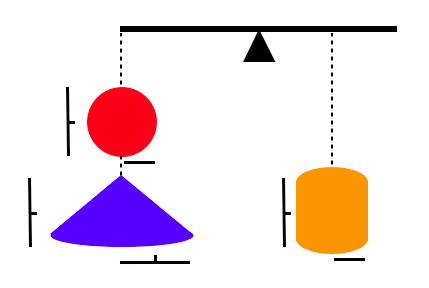
\includegraphics [scale=0.4] {archimedes1.png} \end{center}

There are three factors that complicate our calculation:  (i) we now have a single cone with radius $2r$ and height $2r$ (because it's doubled in both radius and height the cone's volume is increased by a factor of $2^3$), (ii) the sphere and cone are twice as far from the fulcrum as the cylinder, and (iii) the cylinder is made out of something denser than the other objects (four times more dense).

Let $\pi r^3$ be one unit of volume, then the volumes are

\[ sphere =   \frac{4}{3} \]
\[ cone =     \frac{1}{3} \times 8 = \frac{8}{3} \]
\[ cylinder = 2 \]

That's $12/3 = 4$ for the sphere plus cone, and furthermore they count double since they are twice the distance from the fulcrum, giving $8$ in our volume units.  So the left side should be $4 \times$ the weight on the right side.  However, we are told that the density of the material for the cylinder was four times that of the objects on the left.  Hence, it all balanced.

I looked up some densities to try to guess what Archimedes used:

\begin{center}
  \begin{tabular}{ | l | l | } \hline
   sand & $2.80$  \\ \hline
   copper     & $8.63$  \\ \hline
   silver  & $10.40$ \\ \hline
   gold     & $19.30$  \\ \hline
   marble  & $2.56$ \\ \hline
   \end{tabular}
\end{center}

How about marble and silver?

\end{document}  